\PassOptionsToPackage{unicode=true}{hyperref} % options for packages loaded elsewhere
\PassOptionsToPackage{hyphens}{url}
\PassOptionsToPackage{dvipsnames,svgnames*,x11names*}{xcolor}
%
\documentclass[10pt,ignorenonframetext,]{beamer}
\usepackage{pgfpages}
\setbeamertemplate{caption}[numbered]
\setbeamertemplate{caption label separator}{: }
\setbeamercolor{caption name}{fg=normal text.fg}
\beamertemplatenavigationsymbolsempty
% Prevent slide breaks in the middle of a paragraph:
\widowpenalties 1 10000
\raggedbottom
\setbeamertemplate{part page}{
\centering
\begin{beamercolorbox}[sep=16pt,center]{part title}
  \usebeamerfont{part title}\insertpart\par
\end{beamercolorbox}
}
\setbeamertemplate{section page}{
\centering
\begin{beamercolorbox}[sep=12pt,center]{part title}
  \usebeamerfont{section title}\insertsection\par
\end{beamercolorbox}
}
\setbeamertemplate{subsection page}{
\centering
\begin{beamercolorbox}[sep=8pt,center]{part title}
  \usebeamerfont{subsection title}\insertsubsection\par
\end{beamercolorbox}
}
\AtBeginPart{
  \frame{\partpage}
}
\AtBeginSection{
  \ifbibliography
  \else
    \frame{\sectionpage}
  \fi
}
\AtBeginSubsection{
  \frame{\subsectionpage}
}
\usepackage{lmodern}
\usepackage{amssymb,amsmath}
\usepackage{ifxetex,ifluatex}
\usepackage{fixltx2e} % provides \textsubscript
\ifnum 0\ifxetex 1\fi\ifluatex 1\fi=0 % if pdftex
  \usepackage[T1]{fontenc}
  \usepackage[utf8]{inputenc}
  \usepackage{textcomp} % provides euro and other symbols
\else % if luatex or xelatex
  \usepackage{unicode-math}
  \defaultfontfeatures{Ligatures=TeX,Scale=MatchLowercase}
\fi
\usetheme[]{Singapore}
\usefonttheme{serif}
% use upquote if available, for straight quotes in verbatim environments
\IfFileExists{upquote.sty}{\usepackage{upquote}}{}
% use microtype if available
\IfFileExists{microtype.sty}{%
\usepackage[]{microtype}
\UseMicrotypeSet[protrusion]{basicmath} % disable protrusion for tt fonts
}{}
\IfFileExists{parskip.sty}{%
\usepackage{parskip}
}{% else
\setlength{\parindent}{0pt}
\setlength{\parskip}{6pt plus 2pt minus 1pt}
}
\usepackage{xcolor}
\usepackage{hyperref}
\hypersetup{
            pdftitle={Klassifikasjon},
            pdfauthor={Stefanie Muff, Institutt for matematiske fag},
            colorlinks=true,
            linkcolor=Maroon,
            filecolor=Maroon,
            citecolor=Blue,
            urlcolor=blue,
            breaklinks=true}
\urlstyle{same}  % don't use monospace font for urls
\newif\ifbibliography
\usepackage{longtable,booktabs}
\usepackage{caption}
% These lines are needed to make table captions work with longtable:
\makeatletter
\def\fnum@table{\tablename~\thetable}
\makeatother
\usepackage{graphicx,grffile}
\makeatletter
\def\maxwidth{\ifdim\Gin@nat@width>\linewidth\linewidth\else\Gin@nat@width\fi}
\def\maxheight{\ifdim\Gin@nat@height>\textheight\textheight\else\Gin@nat@height\fi}
\makeatother
% Scale images if necessary, so that they will not overflow the page
% margins by default, and it is still possible to overwrite the defaults
% using explicit options in \includegraphics[width, height, ...]{}
\setkeys{Gin}{width=\maxwidth,height=\maxheight,keepaspectratio}
\setlength{\emergencystretch}{3em}  % prevent overfull lines
\providecommand{\tightlist}{%
  \setlength{\itemsep}{0pt}\setlength{\parskip}{0pt}}
\setcounter{secnumdepth}{0}

% set default figure placement to htbp
\makeatletter
\def\fps@figure{htbp}
\makeatother

\usepackage{multicol}

\title{Klassifikasjon}
\providecommand{\subtitle}[1]{}
\subtitle{ISTx1003 Statistisk læring og Data Science}
\author{Stefanie Muff, Institutt for matematiske fag}
\date{November 5 og 8, 2021}

\begin{document}
\frame{\titlepage}

\begin{frame}{Anerkjennelse}
\protect\hypertarget{anerkjennelse}{}

\(~\)

Disse slides bygger på slides fra Mette Langaas, 2020.

Takk til Mette for at jeg fikk bruke noen av materialene.

\end{frame}

\begin{frame}{Plan tema ``Klassifikasjon''}
\protect\hypertarget{plan-tema-klassifikasjon}{}

\(~\)

\begin{itemize}
\item
  Læringsmål og ressurser
\item
  Hva er klassifikasjon?
\item
  Trening, validering og testing (3 datasett)
\item
  \(k\)-nærmeste nabo (KNN): en intuitiv metode
\item
  Forvirringsmatrise og feilrate for å evaluere metoden
\item
  Logistisk regresjon
\end{itemize}

\end{frame}

\begin{frame}{Læringsmål}
\protect\hypertarget{luxe6ringsmuxe5l}{}

\begin{itemize}
\item
  kunne forstå hva klassifikasjon går ut på og kjenne situasjoner der
  klassifikasjon vil være en aktuell metode å bruke
\item
  kjenne begrepene treningssett, valideringssett og testsett og forstå
  hvorfor vi lager dem og hva de skal brukes til
\item
  vite hva en forvirringsmatrise er, og kjenne til begrepene
  \emph{feilrate} (error rate) og \emph{nøyaktighet} (accuracy)
\item
  forstå tankegangen bak \(k\)-nærmeste nabo-klassifikasjon, valg av
  \(k\)
\item
  kjenne til modellen for logistisk regresjon, og kunne tolke de
  estimerte koeffisientene
\item
  forstå hvordan vi utfører klassifikasjon i Python
\item
  kunne besvare problem 2 av prosjektoppgaven
\end{itemize}

\end{frame}

\begin{frame}{Læringsressurser}
\protect\hypertarget{luxe6ringsressurser}{}

\vspace{2mm}

\(~\)

Tema Klassifikasjon:

\vspace{2mm}

\begin{itemize}
\item
  \textbf{Kompendium}: Klassifikasjon (pdf og html, by Mette Langaas)
\item
  \textbf{Korte videoer}: (by Mette Langaas)

  \begin{itemize}
  \tightlist
  \item
    Introduksjon og \(k\)-nærmeste nabo klassifiiasjon (10:58)
  \item
    Logistisk regresjon (14:17)
  \end{itemize}
\item
  Denne forelesningen
\item
  \textbf{Disse slides} med notater
\end{itemize}

\end{frame}

\begin{frame}{Klassifikasjon -- hva er det?}
\protect\hypertarget{klassifikasjon-hva-er-det}{}

\begin{itemize}
\item
  Mål:

  \begin{itemize}
  \item
    tilordne en ny observasjon til en av flere \emph{kjente} klasser
  \item
    lage en klassifikasjonsregel
  \item
    estimere sannsynligheten for at en ny observasjon tilhører de ulike
    klassene
  \end{itemize}
\end{itemize}

\vspace{2mm}

For hver av de uavhengige observasjonene \(i=1,\ldots,n\) har vi

\begin{itemize}
\tightlist
\item
  Forklaringsvariabler \((x_{1i},x_{2i},\ldots,x_{pi})\)
\item
  En kategorisk responsvariablel \(y_i\).
\end{itemize}

\end{frame}

\begin{frame}

\begin{block}{Eksempler I}

\vspace{2mm}

\begin{itemize}
\tightlist
\item
  Hvilke tall er handskrevet på brev? Og hva er sannsynligheten for de
  ulike tallene (=klasser)? \vspace{2mm}
\end{itemize}

\centering

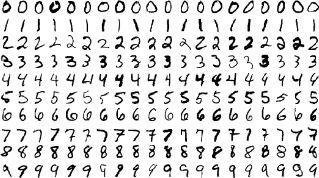
\includegraphics[width=0.5\textwidth,height=\textheight]{mnist.jpeg}

\vspace{4mm}

\flushleft

\begin{itemize}
\tightlist
\item
  Kommer en gitt kunde til å betale tilbake lånet sitt?
\end{itemize}

\vspace{2mm}

\begin{itemize}
\tightlist
\item
  Prognose om noen blir syk (hjertesykdom, kreft\ldots{}) og
  sannsynligheten for det.
\end{itemize}

\end{block}

\end{frame}

\begin{frame}

\begin{block}{Eksempler II}

\(~\)

Problem 2 i prosjektet:

\vspace{2mm}

``Spam eller ham?'' Spam filter: Klassifikasjon for å finne ut om en
e-post er spam eller ikke (=``ham'').

\vspace{2mm}

Binær: Respons variable er ``ja''/``nei'' (1/0).

\vspace{2mm}

\end{block}

\end{frame}

\begin{frame}

\begin{block}{Syntetisk eksempel}

\(~\)

\begin{itemize}
\tightlist
\item
  Et datasett med folgende struktur: \((x_{1i},x_{2i},y_i)\).
  \vspace{2mm}
\end{itemize}

\begin{center}\includegraphics[width=0.6\linewidth]{2Klassifikasjon_files/figure-beamer/unnamed-chunk-1-1} \end{center}

Spørsmål vi vil besvare: Hva er de beste klassifikasjonsgrensene?

\end{block}

\end{frame}

\begin{frame}

\begin{block}{Et reelt eksempel}

\vspace{2mm}

\includegraphics[width=0.9\textwidth,height=\textheight]{flipper.png}

\tiny

\textcolor{gray}{https://github.com/allisonhorst/palmerpenguins}

\end{block}

\end{frame}

\begin{frame}{Data}
\protect\hypertarget{data}{}

\vspace{2mm}

Datasett: \((x_{1i},x_{2i},\ldots, x_{pi},y_i)\)

\vspace{2mm}

Vi må dele datasettet i tre deler:

\vspace{2mm}

\begin{itemize}
\tightlist
\item
  Treningsdata
\item
  Valideringsdata
\item
  Testdata
\end{itemize}

\vspace{5mm}


\includegraphics{datasett.png}

\vspace{2mm}

Hvorfor det?

\end{frame}

\begin{frame}{Trening-, validering- og testsett for syntetiske data}
\protect\hypertarget{trening--validering--og-testsett-for-syntetiske-data}{}

\begin{center}\includegraphics[width=0.9\linewidth]{2Klassifikasjon_files/figure-beamer/unnamed-chunk-2-1} \end{center}

\end{frame}

\begin{frame}{\(k\)-nærmeste-nabo-klassifikasjon}
\protect\hypertarget{k-nuxe6rmeste-nabo-klassifikasjon}{}

\(~\)

For å \emph{finne} klassifikasjonsreglen bruker vi bare treningsdataene.

\(~\)

Algoritmen:

\begin{enumerate}
[1)]
\item
  Ny observasjon: \(x_0=(x_{1,0}, x_{2,0} , \ldots , x_{p,0})\) .
  Hvilken klasse bør denne klassifiseres til?
\item
  Finn de \(k\) nærmeste naboene til observasjonen i treningssettet.
\item
  Sannsynligheten for at den nye observasjonen tilhører klasse 1 anslår
  vi er andelen av de \(k\) nærmeste naboene som har tilhører klasse 1.
  Ditto for de andre klassene.
\item
  Klassen til den nye observasjonen er den som har størst sannsynlighet.
  Det blir det samme som å bruke flertallsavstemming.
\end{enumerate}

\end{frame}

\begin{frame}{\(k\)-nærmeste-nabo-klassifikasjon}
\protect\hypertarget{k-nuxe6rmeste-nabo-klassifikasjon-1}{}

\vspace{5mm}

Tre sp\oe rsm\aa l: \vspace{5mm}

\begin{itemize}
\tightlist
\item
  Hva betyr ``n\ae rmest''? Vi trenger en definision av avstand.
\end{itemize}

\vspace{1.5cm}

\begin{itemize}
\tightlist
\item
  Hvilke verdier kan \(k\) ha?
\end{itemize}

\vspace{1.5cm}

\begin{itemize}
\tightlist
\item
  Hvordan bestemmer vi \(k\)?
\end{itemize}

\end{frame}

\begin{frame}

\begin{block}{Hva betyr nærmest?}

\vspace{2mm}

Nærmest er definert ved å bruke Euklidsk avstand.

\centering

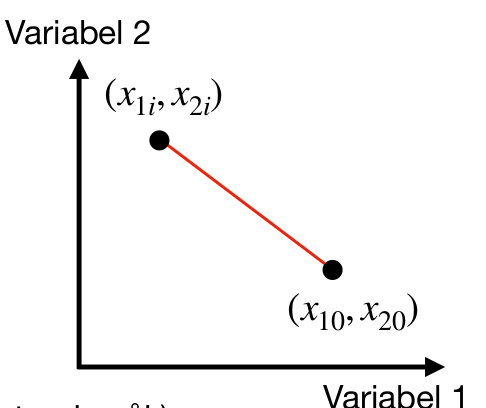
\includegraphics[width=0.4\textwidth,height=\textheight]{avstand.png}

\flushleft

Euklidsk avstand: \[D_E(i,0)=\sqrt{\sum_{j=1}^p (x_{ji}-x_{j0})^2 }\]

Andre avstandsm\aa l kan ogs\aa  ~brukes, men Euklidsk avstand er mest
vanlig.

\end{block}

\end{frame}

\begin{frame}

\begin{block}{N\ae rmeste naboer}

\vspace{5mm}

\begin{center}\includegraphics[width=0.6\linewidth]{2Klassifikasjon_files/figure-beamer/unnamed-chunk-3-1} \end{center}

\end{block}

\end{frame}

\begin{frame}

\begin{block}{N\ae rmeste naboer}

\vspace{5mm}

\begin{center}\includegraphics[width=0.6\linewidth]{2Klassifikasjon_files/figure-beamer/unnamed-chunk-4-1} \end{center}

\end{block}

\end{frame}

\begin{frame}

\begin{block}{Tegn klassegrenser}

\vspace{5mm}

\begin{center}\includegraphics[width=0.6\linewidth]{2Klassifikasjon_files/figure-beamer/unnamed-chunk-5-1} \end{center}

\end{block}

\end{frame}

\begin{frame}

\begin{block}{Hvordan ser klassegrensene ut?}

\(~\)

Husk: Vi bruker treningssettet for å finne klassifikasjonsreglen:

\(~\)

\begin{center}\includegraphics[width=0.7\linewidth]{2Klassifikasjon_files/figure-beamer/unnamed-chunk-6-1} \end{center}

\end{block}

\end{frame}

\begin{frame}

\begin{block}{Hvordan ser klassegrensene ut?}

\(~\) Svar: It depends!

\begin{center}\includegraphics[width=0.7\linewidth]{2Klassifikasjon_files/figure-beamer/knnplot-1} \end{center}

\end{block}

\end{frame}

\begin{frame}

\begin{block}{Men vent\ldots{} hvordan velger vi \(k\) da?}

\(~\)

Vi så jo at

\begin{itemize}
\tightlist
\item
  Hvis man velger \(k\) for lite, da blir grensen \emph{for fleksibel}.
\end{itemize}

\(~\)

Men:

\begin{itemize}
\tightlist
\item
  Hvis man velger \(k\) for stor, kan grensen bli \emph{for ufleksibel}.
\end{itemize}

\(~\)

Det er noe som kalles en trade-off, og vi skal bruk valideringssettet
for å få en idé om kvaliteten i klassifikasjonen.

\end{block}

\end{frame}

\begin{frame}

\begin{block}{Forvirringsmatrise}

\(~\)

Forvirringsmatrise med to klasser:

\centering

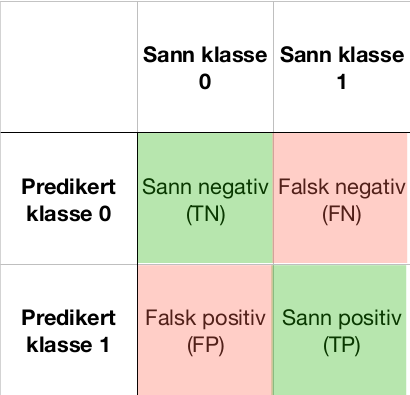
\includegraphics[width=0.35\textwidth,height=\textheight]{forvirringsmatrise.png}\\
\scriptsize (Fra Mette Langaas)

\normalsize

\(~\)

\flushleft

\begin{itemize}
\tightlist
\item
  \textbf{Feilrate}: andel feilklassifiserte observasjoner.
\end{itemize}

\(~\)

\begin{itemize}
\tightlist
\item
  Derfor: Vi velger den \(k\) som minimerer feilraten på
  \emph{valideringssettet} (ikke trainingssettet!).
\end{itemize}

\end{block}

\end{frame}

\begin{frame}

Marker og tell antall gale klassifiseringer på valideringssettet
(\(k=1\)):

\begin{center}\includegraphics[width=0.7\linewidth]{2Klassifikasjon_files/figure-beamer/knnplot2-1} \end{center}

\end{frame}

\begin{frame}

Igjen, men nå med \(k=99\):

\begin{center}\includegraphics[width=0.7\linewidth]{2Klassifikasjon_files/figure-beamer/knnplot3-1} \end{center}

\end{frame}

\begin{frame}

\begin{block}{Feilrate i valideringssettet}

\(~\)

Det kan vi nå systematisk gjøre med alle \(k=1,3,\ldots\), \(k\leq n\):

\vspace{5mm}

\begin{center}\includegraphics[width=0.7\linewidth]{2Klassifikasjon_files/figure-beamer/knn_validation-1} \end{center}

\end{block}

\end{frame}

\begin{frame}

Klassegrensene ser ganske likt ut for \(k=15\) og \(k=99\)
(\(k\geq 15\)):

\begin{center}\includegraphics[width=0.7\linewidth]{2Klassifikasjon_files/figure-beamer/knnplot4-1} \end{center}

\end{frame}

\begin{frame}{Data}
\protect\hypertarget{data-1}{}

\vspace{2mm}

Husk at vi hadde \emph{tre} deler i datasettet:

\vspace{2mm}

\begin{itemize}
\tightlist
\item
  \textbf{Treningssett}: For å lage en klassifikasjonsregel
\item
  \textbf{Valideringssett}: For å finne på optimale hyperparametere
\item
  \textbf{Testsett}: For å evaluere regelen på fremtidige data
\end{itemize}

\vspace{5mm}


\includegraphics{datasett.png}

\vspace{2mm}

Nå kan vi bruke testsettet for å \emph{finne feilraten} for fremtidige
data.

\end{frame}

\begin{frame}

Feilraten på testsettet for KNN med \(k=15\) (egentlig er \(k=31\) best,
men det gjør ikke en stor forskjell):

\begin{center}\includegraphics[width=0.6\linewidth]{2Klassifikasjon_files/figure-beamer/knnplot5-1} \end{center}

Feilraten er 0.09.

\end{frame}

\begin{frame}[fragile]{\(k\)-nærmeste nabo klassifikasjon i Python}
\protect\hypertarget{k-nuxe6rmeste-nabo-klassifikasjon-i-python}{}

\texttt{knaboer\ =\ np.arange(1,199,step=2)}

\texttt{val\_feilrate\ =\ np.empty(len(knaboer))}

\texttt{for\ i,k\ in\ enumerate(knaboer):}\\
\(~\) \texttt{knn\ =\ KNeighborsClassifier(n\_neighbors=k,p=2)}\\
\(~\)
\texttt{knn.fit(df\_tren{[}{[}\textquotesingle{}x1\textquotesingle{},\textquotesingle{}x2\textquotesingle{}{]}{]},\ df\_tren{[}\textquotesingle{}y\textquotesingle{}{]})}\\
\(~\)
\texttt{val\_feilrate{[}i{]}\ =\ 1-knn.score(df\_val{[}{[}‘x1\textquotesingle{},\textquotesingle{}x2\textquotesingle{}{]}{]},\ df\_val{[}\textquotesingle{}y\textquotesingle{}{]})}

\(~\)

Se prosjektoppgaven for mer Python kode.

\end{frame}

\begin{frame}{Plan tema ``Klassifikasjon''}
\protect\hypertarget{plan-tema-klassifikasjon-1}{}

\(~\)

\begin{itemize}
\item
  Læringsmål og ressurser
\item
  Hva er klassifikasjon?
\item
  Trening, validering og testing (3 datasett)
\item
  \(k\)-nærmeste nabo (KNN): en intuitiv metode
\item
  Forvirringsmatrise og feilrate for å evaluere metoden
\item
  Logistisk regresjon
\end{itemize}

\end{frame}

\begin{frame}{Logistisk regresjon - mål}
\protect\hypertarget{logistisk-regresjon---muxe5l}{}

\(~\)

\begin{itemize}
\tightlist
\item
  Forstå modellen
\end{itemize}

\vspace{2mm}

\begin{itemize}
\tightlist
\item
  Tolke estimerte koeffisienter
\end{itemize}

\vspace{2mm}

\begin{itemize}
\tightlist
\item
  Hypotesetest og \(p\)-verdi
\end{itemize}

\vspace{2mm}

\begin{itemize}
\tightlist
\item
  Velge mellom modeller
\end{itemize}

\vspace{2mm}

\begin{itemize}
\tightlist
\item
  Kunne utføre dette i Python
\end{itemize}

\end{frame}

\begin{frame}{Logistisk regresjon}
\protect\hypertarget{logistisk-regresjon}{}

\(~\)

\begin{itemize}
\tightlist
\item
  Kan bare handtere \emph{to klasser} \(y_i \in \{0,1\}\).
\end{itemize}

\(~\)

\begin{itemize}
\tightlist
\item
  Vi antar at \(Y_i\) har en \textbf{Bernoulli fordeling} med
  suksessannsynlighet \(p_i\), derfor:
\end{itemize}

\[y_i = \begin{cases} 1 \text{ med sannsynlighet } p_i, \\ 0 \text{ med sannsynlighet } 1-p_i. \end{cases}\]

\(~\)

\begin{itemize}
\tightlist
\item
  \textbf{Mål}: For forklaringsvariabler
  \((x_{1i},x_{2i},\ldots,x_{pi})\) vi vil estimere
  \(p_i = \text{Pr}(y_i=1 \mid x_1,\ldots,x_p)\).
\end{itemize}

\end{frame}

\begin{frame}[fragile]

\begin{block}{Eksempel: Kredittkort data}

\vspace{2mm}

Datasettet \texttt{Default} er tatt fra her:
\url{https://rdrr.io/cran/ISLR/man/Credit.html}

\vspace{2mm}

\textbf{Mål} : forutsi om en person ikke betaler kredittkortregning
(``person defaults''), avhengig av årsinntekten (income) og balansen på
kredittkortet (balance).

\textcolor{orange}{Orange: default=yes},
\textcolor{blue}{blue: default=no}.

\centering
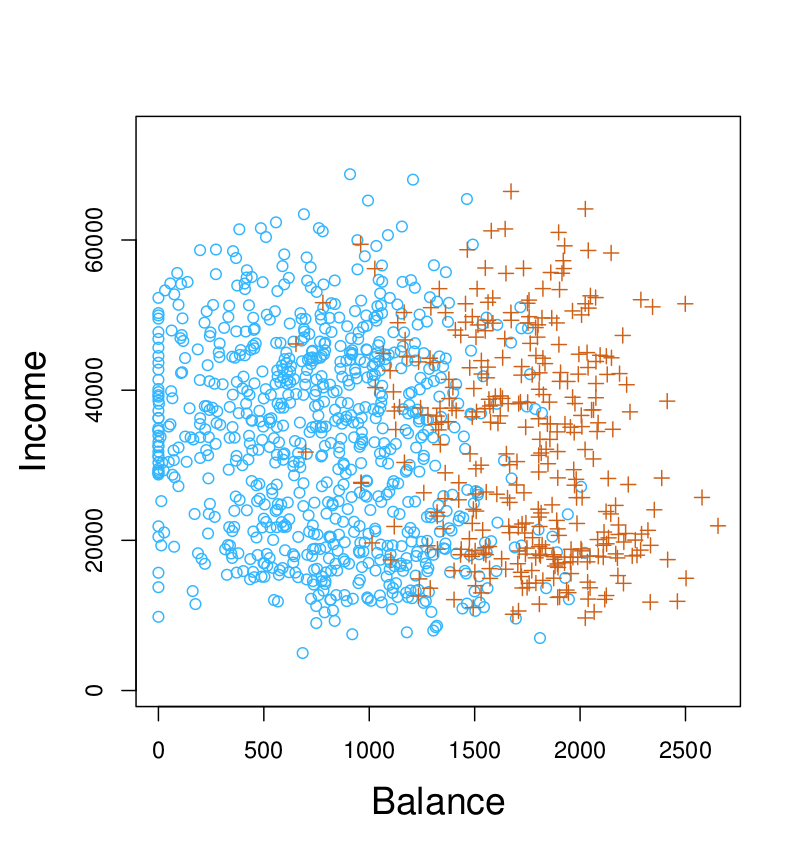
\includegraphics[width=0.5\textwidth,height=\textheight]{4.1a.png}

\end{block}

\end{frame}

\begin{frame}

Det ser ut som at ``Balance'' er en ganske god forklarende variabel til
Default (nei/ja).

\(~\)

\begin{center}\includegraphics[width=0.95\linewidth]{2Klassifikasjon_files/figure-beamer/unnamed-chunk-8-1} \end{center}

\end{frame}

\begin{frame}[fragile]

\begin{block}{Kan vi bare bruke linear regresjon for binær
klassifikasjon?}

\vspace{1mm}

For en binær responsvariabel \(Y =\) \texttt{yes} or \texttt{no}, og
forklaringsvariabler \(X\) bruker vi vannligvis en \emph{dummy encoding}
:

\[Y = \left\{ \begin{array}{ll}
0 & \text{hvis  } \texttt{no} \ , \\
1 & \text{hvis  } \texttt{yes} \ .
\end{array} \right.\]

\vspace{6mm}

\begin{center}\includegraphics[width=0.6\linewidth]{2Klassifikasjon_files/figure-beamer/unnamed-chunk-9-1} \end{center}

\end{block}

\end{frame}

\begin{frame}

\begin{itemize}
\item
  Kunne vi da ikke bare formulere en linear regresjonsmodell for \(Y\)
  vs. \(X\)?
\item
  Vi kunne jo klassifisere responsen som ``ja'' (1) hvis
  \(\hat{Y}> 0.5\).
\end{itemize}

\vspace{2mm}

\begin{itemize}
\tightlist
\item
  Problemet med linear regresjon: Vi kan forutsi \(Y<0\) eller \(Y>1\)
  med modellen, men en sannsynlighet er alltid mellom 0 og 1.
\end{itemize}

\(~\)

For kredittortdatasettet: \vspace{-2mm}

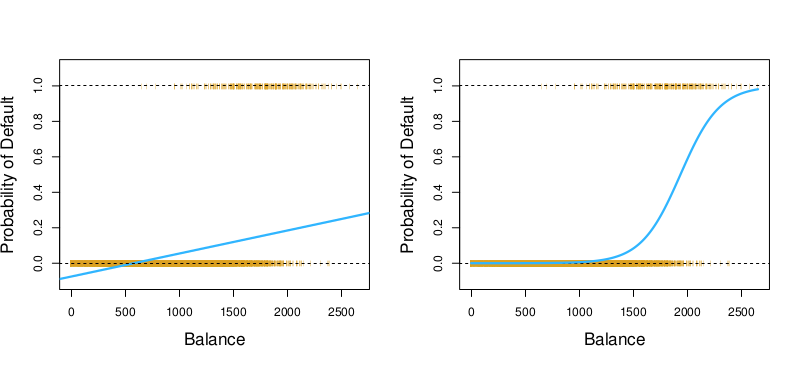
\includegraphics{4.2.png}

\end{frame}

\begin{frame}

\begin{block}{Vi trenger logistisk regresjon!}

\(~\)

\begin{center}\includegraphics[width=0.8\linewidth]{2Klassifikasjon_files/figure-beamer/unnamed-chunk-10-1} \end{center}

\end{block}

\end{frame}

\begin{frame}

\begin{block}{Enkel logistisk regresjon}

\(~\)

\begin{itemize}
\tightlist
\item
  Vi antar at responsen \(Y_i\) er binomisk fordelt med
  suksessannsynlighet \(p_i\)
\end{itemize}

\(~\)

\begin{itemize}
\tightlist
\item
  \textbf{Ideen}: å koble \(p_i\) sammen med forklaringsvariablen med en
  logistisk funksjon:
\end{itemize}

\[p_i = \frac{\exp(\beta_0 + \beta_1 x_{1i})}{1+ \exp(\beta_0 + \beta_1 x_{1i})} \ .\]
\(~\)

\begin{itemize}
\tightlist
\item
  Denne verdien \(p_i\) er alltid mellom 0 og 1, som den skal være.
\end{itemize}

\vspace{2mm}

\(~\)

\(~\)

\end{block}

\end{frame}

\begin{frame}

\begin{block}{Klassifikasjonsregel}

\(~\)

I kredittkorteksempelet er \(x_{1i}\) balansen til person \(i\).

\(~\)

Klassifikasjonsregel: \(p\geq 0.5\) vs \(p<0.5\).

\(~\)

\begin{center}\includegraphics[width=0.8\linewidth]{2Klassifikasjon_files/figure-beamer/unnamed-chunk-11-1} \end{center}

\end{block}

\end{frame}

\begin{frame}

\begin{block}{Enkel logistisk regresjon med Python}

\(~\)

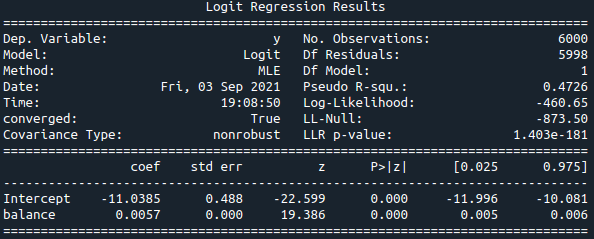
\includegraphics{default_enkelt.png}

\end{block}

\end{frame}

\begin{frame}

\begin{block}{Tolkning av \(\beta_1\): odds}

\(~\)

\begin{itemize}
\tightlist
\item
  Odds er definert som ratioen mellom sannsynlighet for suksess (\(p\))
  og fiasko (\(1-p\)): \[odds = \frac{p}{1-p}\]
\end{itemize}

\(~\)

\begin{itemize}
\tightlist
\item
  Noen eksempler (og zoom poll):
\end{itemize}

\(~\)

\vspace{5mm}

\(~\)

\(~\)

\begin{itemize}
\tightlist
\item
  I logistisk regresjon: Hvis vi øker verdien til kovariaten fra
  \(x_{i1}\) til \(x_{i1} + 1\) så blir den nye oddsen lik den gamle
  multiplisert med \(e^{\beta_1}\).
\end{itemize}

\end{block}

\end{frame}

\begin{frame}[fragile]

\begin{block}{Enkel logistisk regresjon}

\(~\)

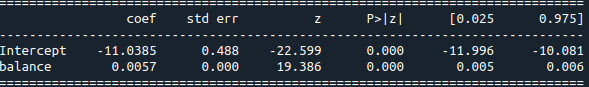
\includegraphics{default_enkelt2.png}

\(~\)

\(~\)

\begin{itemize}
\tightlist
\item
  \(\beta_0=-11.0385\), \(\beta_1=0.0057\).
\end{itemize}

\vspace{3mm}

\begin{itemize}
\tightlist
\item
  \(e^{0.0057}=1.0057\): Hvis \texttt{balance} øker med 1, går oddsen
  opp en \emph{faktor} 1.0057.
\end{itemize}

\vspace{3mm}

\begin{itemize}
\tightlist
\item
  \(e^{0.0057\cdot 100}=1.768\): Hvis \texttt{balance} øker med 100, går
  oddsen opp en \emph{faktor} 1.769.
\end{itemize}

\vspace{3mm}

\begin{itemize}
\tightlist
\item
  Husk at \(H_0: \beta_1=0\) versus \(H_1: \beta_1\neq 0\). Her har vi
  \(p<0.001\) for testen, derfor forkaster vi \(H_0\).
\end{itemize}

\vspace{10mm}

\end{block}

\end{frame}

\begin{frame}

\begin{block}{Logistisk regresjon med flere forklaringsvariabler}

\(~\)

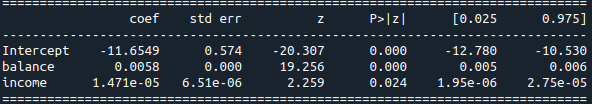
\includegraphics{default_multiple.png}

\(~\)

\begin{itemize}
\tightlist
\item
  Nytt:
  \[p_i = \frac{\exp(\beta_0 + \beta_1 x_{1i} + \beta_2 x_{2i})}{ 1 + \exp(\beta_0 + \beta_1 x_{1i} + \beta_2 x_{2i})}\]
\end{itemize}

\vspace{2mm}

\begin{itemize}
\tightlist
\item
  Tolkning av \(\beta_1\) og \(\beta_2\)?
\end{itemize}

\vspace{2mm}

\begin{itemize}
\tightlist
\item
  \(p\)-verdi?
\end{itemize}

\end{block}

\end{frame}

\begin{frame}[fragile]

\begin{block}{Hvilken model er bedre?}

\vspace{2mm}

\begin{itemize}
\tightlist
\item
  For klassifikasjonen, skal vi velge modellen med bare \texttt{balance}
  eller med \texttt{balance\ +\ income}?
\end{itemize}

\vspace{2mm}

\begin{itemize}
\tightlist
\item
  Ideen: Skjekk feilrate på valideringssettet!
\end{itemize}

\vspace{2mm}

\begin{itemize}
\tightlist
\item
  Husker du bruk av forvirringsmatrise?
\end{itemize}

\vspace{2mm}

\begin{itemize}
\tightlist
\item
  Det er resultatene fra modellene:
\end{itemize}

\begin{longtable}[]{@{}lcc@{}}
\toprule
& pred:no & pred:yes\tabularnewline
\midrule
\endhead
true:no & 1923 & 10\tabularnewline
true:yes & 52 & 15\tabularnewline
\bottomrule
\end{longtable}

\begin{longtable}[]{@{}lcc@{}}
\toprule
& pred:no & pred:yes\tabularnewline
\midrule
\endhead
true:no & 1924 & 9\tabularnewline
true:yes & 50 & 17\tabularnewline
\bottomrule
\end{longtable}

\begin{itemize}
\tightlist
\item
  Feilratene er derfor0.031 (enkel modell) og 0.0295 (multippel modell)
\end{itemize}

\end{block}

\end{frame}

\begin{frame}

\begin{block}{Feilrate testsett}

\(~\)

Til slutten kan vi sjekke feilraten på testsettet -- dette settet har vi
enda ikke brukt.

\(~\)

Her finner vi 0.0245

\end{block}

\end{frame}

\begin{frame}[fragile]

\begin{block}{Python code}

\(~\)

\texttt{formel=\textquotesingle{}y\ \textasciitilde{}\ balance\ +\ income\textquotesingle{}}\\
\texttt{modell\ =\ smf.logit(formel,data=df)}~\\
\texttt{resultat\ =\ modell.fit()}~\\
\texttt{resultat.summary()}~\\
\texttt{print(np.exp(resultat.params))}

\(~\)

\texttt{cutoff\ =\ 0.5}\\
\texttt{test\_pred\ =\ resultat.predict(exog\ =\ df\_test)}~\\
\texttt{y\_testpred\ =\ np.where(test\_pred\ \textgreater{}\ cutoff,\ 1,\ 0)}~\\
\texttt{y\_testobs\ =\ df\_test{[}\textquotesingle{}y\textquotesingle{}{]}}~\\
\texttt{print("Feilrate:",\ 1-accuracy\_score(y\_true=y\_testobs,}~\\
\(~\) \texttt{y\_pred=y\_testpred,normalize=True))}

\end{block}

\end{frame}

\begin{frame}{Videre denne uken}
\protect\hypertarget{videre-denne-uken}{}

\(~\)

\begin{itemize}
\tightlist
\item
  Se på videoene om Klyngeanalyse og K-gjennomsnitt (vent med videoen om
  hierarkisk klyngeanalyse).
\end{itemize}

\(~\)

\begin{itemize}
\tightlist
\item
  Les i kompendiet
\end{itemize}

\(~\)

\begin{itemize}
\tightlist
\item
  Begynn å jobbe med prosjektoppgavene
\end{itemize}

\(~\)

\begin{itemize}
\tightlist
\item
  Se her for mer informasjon:
  \url{https://wiki.math.ntnu.no/istx1003/2021h/start}
\end{itemize}

\end{frame}

\end{document}
